\icode{E-MD-CA-L4-261121-001}
如图所示，粗糙的水平地面上静置一个足够长的木板\( A \)，\( A \) 的质量为 \SI{1}{kg}，在 \( A \) 的右端\( L = \SI{2}{m} \) 处每隔 \SI{0.2}{m}设置一个挡板，从左往右依次标记为 1，2，3，\(\cdots\)， \( n(n \to \infty) \)。现把质量为 \SI{1}{kg} 的物块 \( B \) 以 \( v_0 = \SI{4}{m/s} \) 的初速度滑上 \( A \) 的左端，同时对 \( A \) 施加水平向右的推力 \( F = \SI{4}{N} \)，已知 \( B \) 与 \( A \)，\( A \) 与水平地面之间动摩擦因数均为 \( \mu = 0.2 \)，若木板 \( A \) 每次与挡板碰撞后都以碰撞前的速率反弹，且每次与挡板碰后立即撤离该被碰挡板，物块 \( B \) 始终没有与挡板相碰，\( B \) 也始终没有滑离木板 \( A \)，设最大静摩擦力等于滑动摩擦力，重力加速度 \( g \) 取 \SI{10}{m/s^2}。求:
\begin{enumerate}
	\item \( B \) 滑上 \( A \) 时，\( A \)，\( B \) 的加速度分别为多大;
	\item 从 \( B \) 滑上 \( A \) 到 \( A \) 与挡板 1 碰撞的过程中，\( B \) 的位移大小;
	\item \( B \) 在 \( A \) 上面滑行时，\( B \) 相对于 \( A \) 滑行的总位移 (结果可以用分数表示)。
\end{enumerate}

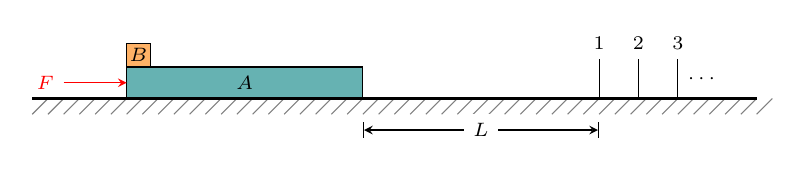
\begin{tikzpicture}[>=stealth,font=\scriptsize]
	\draw[fill=teal!60] (0,0) rectangle(3,.4)node[midway]{\(A\)};
	\draw[fill=orange!60] (0,.4) rectangle(.3,.7)node[midway]{\(B\)};
	\draw[red,->] (-.8,.2)node[left]{\(F\)}--++(.8,0);
	\foreach \x/\num in {6/1,6.5/2,7/3}
		\draw (\x,0)--++(0,.5)node[above]{\(\num\)};
	\foreach \x in {-1.2,-1,...,8}
		\draw[gray] (\x,-.2)--++(.2,.2);
	\draw[thick] (-1.2,0)--(8,0);
	\draw[|<->|] (3,-.4)--node[fill=white]{\(L\)}(6,-.4);
	\node at(7.3,.25){\(\cdots\)};
\end{tikzpicture}
\begin{answer}
	（1）\(a_A =\) \,\qty{2}{m/s^2}，\(a_B =\) \,\qty{2}{m/s^2}（2）\(x_B =\) \,\qty{4}{m}（3）\(\Delta x = \frac{64}{21}\) \qty{}{m}
\end{answer}